% =====================================================================
%  What a slice-level benchmark certifies without the pixels
%  Main manuscript, Radiology: Artificial Intelligence (RSNA) format
%  Compiles with stock Overleaf / pdfLaTeX. No shell-escape, no custom
%  class, no exotic packages: geometry, amsmath, graphicx, array,
%  booktabs, siunitx, caption, natbib, hyperref only.
%
%  BIBLIOGRAPHY: refs.bib, in the same folder. Build order on Overleaf is
%  pdfLaTeX -> BibTeX -> pdfLaTeX x2. The citation keys used here are, in
%  alphabetical order:
%    badgeley2019hip, bejnordi2017camelyon16, burduja2020ich,
%    camelyon16leaderboard, chen2025camcsa, colak2021rsnape,
%    degrave2021covid, flanders2020rsnaich, fleiss1971kappa,
%    geirhos2020shortcut, guo2019wsi, gwet2008ac1, holm1979, islam2021pe,
%    jarkman2022generalization, kapoor2023leakage, maierhein2018rankings,
%    ongly2024shortcut, osciiart2020baseline, page2021prisma,
%    rempe2024kspace, roberts2021pitfalls, ruan2021wsi,
%    saha2018radiogenomics, saha2021dukebreastmri, saha2024picai,
%    setio2017luna16, tampu2022leakage, tibrewala2023fastmriprostate,
%    trivialbaselines2026, varoquaux2022failures, wen2020cnn, wilson1927,
%    yagis2021leakage, yan2018deeplesion, yan2018deeplesiongraphs,
%    zech2018pneumonia, zhao2022fastmriplus
%  (osciiart2020baseline is a Kaggle notebook; rempe2024kspace is an arXiv
%   preprint -- both must be cited as such.)
% =====================================================================
\documentclass[11pt,a4paper]{article}

\usepackage[T1]{fontenc}
\usepackage[utf8]{inputenc}
\usepackage[margin=1in]{geometry}
\usepackage{amsmath}
\usepackage{graphicx}
\usepackage{array}
\usepackage{booktabs}
\usepackage{siunitx}
\usepackage[font=small,labelfont=bf]{caption}
\usepackage[numbers,sort&compress]{natbib}
\usepackage[hidelinks]{hyperref}

\sisetup{group-separator={,},group-minimum-digits=4,detect-weight=true}

% Placeholder marker for anything not yet supplied by a source artefact.
\newcommand{\todo}[1]{\textbf{[#1]}}

\setlength{\parskip}{0.4em}
\setlength{\parindent}{0pt}
\renewcommand{\arraystretch}{1.15}

\title{\bfseries What a slice-level benchmark certifies\\
without the pixels:\\[0.15em]
an audit of seven public benchmarks and a pre-registered\\
screen of how often the check is reported}

\author{%
Sathvik Loke,\thanks{Corresponding author: \texttt{sloke@imsa.edu}}\;
Ethan Johnson,\;
Neeraj Movva,\;
Aditya Raut
}
\date{}

\begin{document}
\maketitle

% ---------------------------------------------------------------------
\begin{center}
\small
\begin{tabular}{@{}l@{}}
\textbf{Affiliations}\\[0.3em]
Sathvik Loke, Neeraj Movva --- Illinois Mathematics and Science Academy, Aurora, Ill.\\
Ethan Johnson --- \todo{MISSING: affiliation for Ethan Johnson}\\
Aditya Raut --- \todo{MISSING: affiliation for Aditya Raut}\\[0.4em]
\textbf{E-mail} \texttt{sloke@imsa.edu}, \texttt{ethanthekek21@gmail.com},\\
\texttt{nmovva@imsa.edu}, \texttt{aditya.sraut09@gmail.com}\\[0.4em]
\textbf{Funding} \todo{MISSING: funding statement}\\
\textbf{Conflicts of interest} \todo{MISSING: COI disclosures for all authors}\\
\end{tabular}
\end{center}

% Word counts requested at submission:
% \todo{MISSING: final word count of manuscript body, to be inserted at submission}

\vspace{0.6em}
\hrule
\vspace{0.8em}

% =====================================================================
% NOTE ON LENGTH: this abstract runs ~380 words and the body ~8,200 words.
% Radiology: AI caps the structured abstract near 300 words and original
% research near 3,000. This draft is deliberately complete for co-author
% review; cut to the caps at submission. Do not cut an interval to make room.
\section*{Abstract}
\addcontentsline{toc}{section}{Abstract}

\textbf{Background.} Volumetric images are often labelled and scored one slice at
a time. Shortcut learning, acquisition confounding and the inflation caused by
slice-level splits are documented, and a pixel-free positional baseline is itself
prior art; what is unmeasured is how much of a published number such a baseline
accounts for under a \emph{correct} split, and how often anyone checks.

\textbf{Purpose.} To quantify how much published slice-level performance is
reachable from a benchmark's own label file with no images, to test whether the
evaluation unit changes which method wins, and to estimate how often this
literature reports any such check.

\textbf{Materials and Methods.} Pixel-blind null models requiring only four
commonly published columns --- subject identifier, slice index, label, train/test
assignment --- were fitted on training slices, and the resulting score vector was
read at both the slice and the patient level with subject-clustered bootstrap
intervals. Seven public benchmarks (eight label files) were audited. A
rank-inversion analysis on 21 method configurations across five cohorts compared
between-unit rank disagreement against within-unit resampling noise. A
pre-registered random-sample screen of a frozen \num{9979}-record PubMed frame
(seed 20260729, four independent screeners) estimated reporting prevalence.
Proportions carry Wilson 95\% CIs.

\textbf{Results.} On RSNA 2019 Intracranial Haemorrhage (\num{752802} slices,
\num{18938} patients) one pixel-blind score vector read 0.737 (95\% CI: 0.735,
0.740) per slice and 0.453 (95\% CI: 0.445, 0.461) per patient, an interval
wholly below chance; all six official labels behaved the same way (gaps
0.205--0.307). Against peer-reviewed comparators the median share of the
published margin over chance reached without pixels was 0.469 (IQR: 0.437, 0.490;
$n=9$ benchmark-arms), and two benchmark-arms did not fire at all (LUNA16,
fraction $-0.002$; PI-CAI, positional baseline exactly 0.500 AUROC). Of 250 sampled papers, 91 were included and readable while 44 (32.6\%;
95\% CI: 25.3\%, 40.9\%) could not be obtained; none of the 91 reported a measured
zero-image baseline (0/91, 0.0\%; 95\% CI: 0.0\%, 4.1\%; bounding interval
0.0\%--32.6\%), and none appeared in any of 345 coded records over 300 papers. No
rank inversion survived (0 of 447 pairs), and on three of five cohorts two
disjoint halves of the same subjects ranked methods in opposite orders.

\textbf{Conclusion.} The unit at which a volumetric benchmark is read decides what
its number means; against peer-reviewed numbers a pixel-blind model reached about
half the reported margin over chance, and in a pre-registered sample of the
literature no paper that could be read reported this check.

\vspace{0.6em}

% =====================================================================
\section*{Key Points}

\begin{itemize}\setlength{\itemsep}{0.2em}
\item On \num{18938} patients, one pixel-blind score vector read 0.737 (95\% CI:
0.735, 0.740) per slice and 0.453 (95\% CI: 0.445, 0.461) per patient; nothing
changed but the unit of evaluation.
\item Against peer-reviewed comparators, a model with no pixels reached a median
0.469 (IQR: 0.437, 0.490; $n=9$) of the published margin over chance; on two of
nine benchmark-arms it reached none of it.
\item In a pre-registered random sample, 0 of 91 readable papers reported any
zero-image baseline (bounding interval 0.0\%--32.6\%, because 32.6\% of the
eligible set could not be obtained).
\end{itemize}

\section*{Summary Statement}

A model that never sees a pixel reproduces roughly half of published
slice-level performance on public volumetric benchmarks and collapses to below
chance when the same scores are read per patient, yet no paper that could be
obtained in a pre-registered random sample of this literature reported such a
check, in a sample where a third of eligible papers could not be obtained.

% =====================================================================
\section*{Abbreviations}

AP = average precision;
AUROC = area under the receiver operating characteristic curve;
CI = confidence interval;
CPM = competition performance metric;
DWI = diffusion-weighted imaging;
FROC = free-response receiver operating characteristic;
ICH = intracranial haemorrhage;
IQR = interquartile range;
PI-RADS = Prostate Imaging Reporting and Data System;
PRISMA = Preferred Reporting Items for Systematic Reviews and Meta-Analyses.

\vspace{0.4em}
\hrule
\vspace{0.4em}

% =====================================================================
\section{Introduction}

A three-dimensional acquisition is often labelled slice by slice --- this slice
contains the lesion, that one does not --- and a classifier's performance is then
reported by pooling slices into a single AUROC. The clinical question is almost
always about a patient. The gap between those two things is arithmetic rather
than opinion: a slice-level ranking can be dominated by \emph{where} a slice sits
in the stack, because findings are not uniformly distributed along an organ, and
a score vector that encodes only that geometry ranks slices well and patients
not at all.

None of this is new, and this paper is written on the assumption that the reader
already knows it. Shortcut learning is a named and canonical phenomenon
\citep{geirhos2020shortcut}. In medical imaging specifically, Badgeley et al.\ showed
hip fracture predicted at AUC 0.78 from the radiograph, 0.91 with hospital
process features added, and 0.52 --- chance --- on a test set balanced across
patient and process variables, with scanner model predictable from the
radiograph at AUC 1.00 \citep{badgeley2019hip}; Zech et al.\ documented the same
mechanism across institutions \citep{zech2018pneumonia}; DeGrave et al.\ showed
radiographic COVID-19 models selecting shortcuts over signal
\citep{degrave2021covid}; and Ong Ly et al.\ found across thirteen datasets that
performance is frequently overestimated by up to 20\% through hidden acquisition
biases, releasing an estimator for it \citep{ongly2024shortcut}. On the evaluation unit,
Yagis et al.\ measured that slice-level cross-validation boosted test accuracy by
30\%--55\% and reached about 96\% accuracy on \emph{randomly labelled} data
\citep{yagis2021leakage}, Tampu et al.\ reported the same inflation in OCT
\citep{tampu2022leakage}, and Wen et al.\ found that more than half of surveyed
Alzheimer disease classification papers may have suffered from data leakage
\citep{wen2020cnn,kapoor2023leakage}. Better baselines have already been recommended at
field level \citep{varoquaux2022failures,roberts2021pitfalls}.

\textbf{The central construction of this paper is prior art, and we say so
here rather than in a discussion paragraph.} A public Kaggle notebook on the
RSNA-STR Pulmonary Embolism Detection challenge, ``Baseline with no image''
(October 2020), bins $P(\text{label}\mid\text{relative slice position})$ on the
training set and applies it to the test set with no pixels, scoring 0.33 on the
public leaderboard against 0.44 for a constant predictor \citep{osciiart2020baseline};
that is the same construction, four years earlier. Yan et al., in the paper that
defines the DeepLesion lesion-type task, publish a ``Baseline: Location
feature'' row at 59.7\% eight-class accuracy against their own method's 90.5\%
\citep{yan2018deeplesiongraphs}. And rankings of biomedical image analysis challenges are
already known to be unstable: Maier-Hein et al.\ show that even at Kendall
$\tau$ of 0.74--0.85 critical changes in the ranking may occur
\citep{maierhein2018rankings}, which caps what anyone may claim about rank inversion.

Two things are nevertheless not established anywhere we could find. First, the
prior literature on the evaluation unit measures the cost of a \emph{wrong}
(leaky) split; the question here is what survives a \emph{correct},
patient-disjoint split. This distinction is load-bearing, and every number
reported below was obtained under a subject-disjoint split. Second, nobody has
measured how much of a published slice-level number a pixel-free model accounts
for, nor how often the check is reported at all.

Asking the question turns out to be nearly free, and that is what makes it
scalable. The inputs a positional null needs --- subject identifier, slice index,
label, split assignment --- are exactly the fields most public benchmarks
publish in a CSV with no data-use agreement and no pixels. A benchmark can
therefore be audited by someone who will never be granted its images, on a
laptop, in one command.

This paper reports five things: (a) the slice-versus-patient divergence of a
single pixel-blind score vector, anchored on a benchmark of \num{18938}
patients that needs no published comparator; (b) how much of a published margin
over chance is reachable without pixels, reported as a distribution, including
the benchmarks on which nothing is reachable; (c) a pre-registered estimate of
how often the field reports any such check; (d) a pre-specified test of whether
the evaluation unit changes which method wins, which returned a null; and (e) a
worked case study, a seven-rule reporting protocol and a released tool. Our
contribution is the formalisation, the subject-clustered statistics, the
slice-versus-patient contrast, the prevalence measurement and the instrument ---
not the idea.

% =====================================================================
\section{Materials and Methods}

\subsection{Study design}

This is a methodological and meta-research study on public data and published
records; no patient was recruited and no identifiable data were used.
Institutional review board approval was \todo{MISSING: IRB / ethics statement
and waiver language}. The audit component analyses published label files only;
no pixel data were downloaded for any audited target. The prevalence screen was
pre-registered before any analysis-sample record was read, and its protocol,
codebook, sealed screener files and analysis script are released. The
pre-registration was not deposited in a public registry before screening began,
which is a reportable deviation from our own protocol.

\subsection{The zero-image baseline family}

Five null models were implemented, each fitting on training rows and scoring
test rows: a constant \emph{prevalence} predictor, which is the chance anchor; a
\emph{positional} model, a 20-bin estimate of the probability of the label given
relative slice position; a \emph{volume-size} model, the number of slices in the
volume; a \emph{metadata} model, a depth-limited classification tree over
acquisition and administrative columns; and a \emph{combined} position-plus-metadata
tree, the ceiling reachable with no pixels. Relative
position is $(\text{slice}-\text{min slice in volume})/(\text{max}-\text{min})$,
so volumes of different depth are comparable. The positional baseline is reported
over a 5/10/20/50 bin sweep and alongside a \emph{no-fit} variant,
$-\lvert\text{relative position}-0.5\rvert$, which uses no training data at all;
a result surviving both cannot be a binning artefact.

\subsection{Column discipline}

Two classes of column are excluded from the metadata pool by default:
\emph{outcome-derived} columns, which are the label under another name, and
\emph{image-derived} columns, which break the zero-image premise. The exclusion
is a fallible name heuristic, so every included and excluded column is printed
and written to the run's JSON payload. On PI-CAI, for example, prostate volume
and PSA density were excluded as image-derived and the ISUP, Gleason, PI-RADS and
histopathology fields as outcome-derived, leaving age, serum PSA, centre and
acquisition year.

\subsection{Evaluation and intervals}

Every baseline produces one score vector per test set, read at \emph{both} units:
slice-level AUROC, and patient-level AUROC after aggregating each subject's slice
scores (mean; a maximum-aggregated reading is reported alongside). Intervals are
percentile bootstrap over \emph{subjects} --- a subject drawn twice contributes
all of their slices twice --- with 2,000 replicates unless stated, seeds
recorded, and degenerate replicates counted rather than dropped. The naive
slice-resampled interval is computed as well and reported in the payload,
explicitly labelled as the incorrect one, so the width difference is visible
rather than asserted. On simulated data where the true AUC is available in closed
form (0.6880; 200 datasets of 20 patients $\times$ 15 slices), the
subject-clustered interval covered the truth 91.5\% of the time at a nominal 95\%
with mean width 0.370, while the naive interval covered it 46.5\% of the time
with mean width 0.117 --- a factor of 3.18 narrower.

\subsection{Permutation nulls}

A null model's chance level is not automatically 0.5. Fitting a metadata model
out of fold on a subject-level label makes the rate fitted anti-correlated with
the rate scored, so on a synthetic dataset whose label is by construction
invisible to metadata the metadata baseline measures 0.424, not 0.500. Every
baseline is therefore reported against its own permutation null --- for the
positional model, labels shuffled \emph{within each series}, which preserves
prevalence, subject clustering and stack depth --- and where a permutation cannot
change anything the null is reported as unavailable rather than as $p=1$.

\subsection{The comparison statistic}

\begin{equation}
\text{trivial fraction}=\frac{\text{best zero-image baseline}-\text{chance}}
{\text{published}-\text{chance}}
\end{equation}

with chance $=0.5$ for AUROC and the majority-class rate for multiclass accuracy.
It is a continuous quantity and is reported as one, for every (benchmark,
published comparator) pair, with an interval, and summarised as a distribution.
Rows are not independent --- one paper's table can supply several comparator
systems for one benchmark --- so the primary summary takes each benchmark-arm's
\emph{strongest} published system, the conservative choice, because a stronger
comparator enlarges the denominator and shrinks the fraction. A categorical
verdict (MATCHED / PARTIAL / NOT MATCHED / NON-COMPARABLE) is retained as a
secondary column so this analysis can be reconciled with an earlier one rather
than replacing it silently; it is a descriptive decision rule, not a hypothesis
test, and no $p$ value is claimed from it. The fraction is undefined, and
returned as such, when the published number is at or below chance; values above
1 and below 0 are reported unclipped. Its interval propagates uncertainty in the
\emph{baseline only}, because a publication's sampling distribution is almost
never available, and it is therefore too narrow as a statement about the ratio.

\subsection{The remedy: position-stratified AUROC}

A stratified Mann--Whitney statistic computes AUROC \emph{within} strata of
relative slice position, so only same-position positive/negative pairs
contribute. It removes exactly the share of a slice-level AUROC that stack
geometry paid for, and nothing else. It runs on a paper's own test predictions
and needs no access to the baselines.

\subsection{Benchmark selection}

A dataset entered the audit if the four positional fields could be obtained
without downloading pixel data and without a data-use agreement covering pixels.
Seven benchmarks across eight label files qualified: RSNA 2019 Intracranial
Haemorrhage \citep{flanders2020rsnaich}, fastMRI Prostate (T2 and DWI)
\citep{tibrewala2023fastmriprostate}, DeepLesion \citep{yan2018deeplesion}, fastMRI+ knee
\citep{zhao2022fastmriplus}, Duke Breast Cancer MRI \citep{saha2021dukebreastmri,saha2018radiogenomics}, PI-CAI
\citep{saha2024picai} and LUNA16 \citep{setio2017luna16}. Datasets investigated and
excluded, with reasons, are reported with the results rather than omitted.

\subsection{Does the unit change the ranking?}

One (architecture, initialisation, input condition) cell counts as a method,
scored by its pooled out-of-fold prediction vector, with every method in a cohort
aligned on identical slices of identical subjects. A single joint clustered
bootstrap of 2,000 replicates resamples \emph{subjects} and, from that one draw,
recomputes the slice-level and patient-level AUROC of every method, so both units
and all methods move together and every comparison is paired. Rank disagreement
is $D=1-\tau_b$. The headline is the paired difference
$\delta_u(b)=D_{\text{between}}(b)-D_{\text{within},u}(b)$ computed inside each
replicate; the unit is credited only if $\delta$ lies entirely above zero against
\emph{both} within-unit noise floors. Named inversion pairs must additionally
have both orderings individually excluded from zero after Holm adjustment
\citep{holm1979} over every pair examined at that unit. Stability thresholds
($\tau=0.50$, top-1 reproducibility $=0.50$) and a 200-replicate split-half
reference over disjoint subject halves were fixed in the analysis file before the
cohorts were run. A paired unit $\times$ condition interaction,
$I(a)=d_{\text{agg}}(a)-d_{\text{slice}}(a)$ with architecture $a$ held fixed,
was pre-specified as the low-multiplicity version of the same question. Published
two-unit comparisons were sought by scanning 2,934 open-access full texts through
the Europe PMC API plus the arXiv API and direct leaderboard fetches, of which
2,642 were passed through the same-metric two-column scanner that supplies the
rarity denominators below; a web search tool was unavailable in both passes, so
coverage figures are lower bounds.

\subsection{The worked-example cohorts}

To demonstrate the protocol where every control could be run, we applied it to
our own study of whether MRI phase carries tumour signal beyond magnitude: three
clinical cohorts (prostate T2 $n=67$, prostate DWI $n=45$, breast $n=70$) and
two confound cohorts whose label is an acquisition property rather than a
diagnosis (brain $n=454$ available volumes, label receive-coil count $\geq 16$;
knee $n=96$, label pulse sequence). The rank-inversion arm is run on the subsets for
which every method's per-slice predictions exist, which is 136 brain and 29 knee
subjects, and Table~\ref{tab:rank} reports those counts rather than the roster
sizes. 102 training runs and 456 control runs, five-fold subject-level
cross-validation, seven architectures, two seeds, pooled out-of-fold estimation
with each subject tested exactly once. Reconstructions were validated against the
vendor reference images shipped in the same files: $r=1.000$ for brain and knee,
0.998 for prostate T2, 0.984 for DWI with the low-$b$ volumes magnitude-averaged
as the vendor does, and 0.977 for breast. Every vendor reference in these
releases is a magnitude image, so these validate the magnitude reconstruction
only; the breast reference is itself a temporal-TV-regularised reconstruction of
the same k-space, so that correlation is agreement between two estimators rather
than a ground truth.

\subsection{The pre-registered prevalence screen}

\textbf{Frame.} One frozen PubMed query for deep-learning classification papers
on volumetric modalities reporting a numeric classification metric, 2019-01-01 to
2026-12-31, English, excluding reviews and case reports; executed 2026-07-29,
\num{9979} records retrieved and hashed (SHA-256 \texttt{d611def0\ldots}). The
frozen list governs.

\textbf{Sample.} A seeded permutation (seed 20260729). Positions 1--100 were
screened; ten pilot records at positions 101--110 are permanently excluded
because the protocol author read them. The protocol fixed a target of 75 included
papers and an extension rule --- continue into the reserve in permutation order,
in blocks of 50, until the target is exceeded --- because at $n=75$ a zero count
carries a Wilson upper bound of 4.9\%. The extension fired and stopped at
position 260. A fifth block (positions 261--310) was screened past the stopping
point and is reported throughout as a labelled post-hoc extension, never pooled
into the pre-registered denominator.

\textbf{Extraction.} Two stages: title and abstract, then a Methods-in-full read
with the results tables, any baseline or statistical-analysis subsection, and the
supplement. Every coded field bearing on a result requires a verbatim quote with
its location. Before a paper may be coded as reporting no trivial baseline, the
screener must run fourteen prescribed full-text searches (\emph{baseline, chance,
random, majority, prevalence, constant, trivial, metadata, clinical-only,
clinical model, position, location, slice index, permut}) and record having done
so; a negative without the search is invalid.

\textbf{Endpoints.} The primary endpoint (P1) is the proportion of included
papers reporting at least one \emph{zero-image} baseline with a measured value on
the same metric: a constant/majority-class/prevalence predictor, a positional
model, an acquisition-metadata model, or a permuted-label null. A
clinical-variables-only arm is deliberately excluded from P1 and reported
separately, because a clinical nomogram asks whether imaging adds to clinical
data, not whether the benchmark is separable without information. An assertion
with no number counts as negative. Secondary endpoints cover the evaluation unit,
the split unit, the positional distribution of labels, the unreachable count,
interval practice and positive-count reporting.

\textbf{Unreachable papers are never dropped.} An access ladder was followed in
order and the rung reached recorded. Sci-Hub and equivalent infringing sources
were refused in every block and no bot-detection challenge was circumvented; a
paper reachable only through such a source stayed unreachable. A paper whose
abstract is consistent with inclusion but whose full text could not be obtained
is coded unreachable, enters the flow diagram, and enters two bounding analyses
reported unconditionally. Where unreachable papers exceed 15\% of the eligible
set, the protocol makes the \textbf{bounding interval the headline}. The
direction of the residual bias was stated in advance: paywalled articles skew
toward higher-tier clinical journals, the venues most likely to demand a
comparator arm, so silently dropping them would push P1 downward --- in the
direction that flatters our own hypothesis.

\textbf{Agreement.} Fifteen papers at permutation positions 1--15 were coded
independently by all four screeners, each submitting a sealed file before seeing
any other. Fleiss $\kappa$ \citep{fleiss1971kappa} is primary; the six pairwise Cohen
$\kappa$ are reported alongside. Because the primary flag was expected to be
extremely skewed, raw percent agreement and Gwet AC1 \citep{gwet2008ac1} were
pre-specified in the same table before any coding. Intervals are bootstrap
percentile 95\% over 2,000 resamples, seed 20260729. A remedy was pre-specified
for $\kappa<0.60$ or raw agreement $<90\%$: a documented adjudication round, a
codebook amendment, and re-coding of every already-coded paper.

\textbf{Statistics.} All proportions carry Wilson score 95\% intervals
\citep{wilson1927}, fixed for every proportion before analysis. No significance
test is pre-specified; this is an estimation study. Reporting follows PRISMA 2020
adapted for a random-sample meta-research screen \citep{page2021prisma}.

\subsection{Software}

The audit tool is \texttt{trivialbaselines} v1.0 (MIT licence)
\citep{trivialbaselines2026}, depending on
\texttt{numpy} and \texttt{pandas} and nothing else. The absence of a deep
learning framework is a deliberate property: the premise is that a benchmark can
be audited with no images, no data-use agreement and no GPU, and a reader should
be able to verify that from the dependency list. A \texttt{--self-test} runs
synthetic data with known answers, and every run writes a JSON payload with every
number traceable plus a human-readable card.

% =====================================================================
\section{Results}

\subsection{Slice-level evaluation of volumetric imaging can be substantially
reproduced without pixels}

Every cell in this subsection is our own computation on a published label file.
No published number enters, so no comparability objection and no comparator's
peer-review status touches it.

On the RSNA 2019 Intracranial Haemorrhage official training file ---
\num{752802} slices, \num{21744} series, \num{18938} patients, the benchmark
whose own official metric is per-slice --- a 20-bin estimate of
$P(\text{label}\mid\text{relative slice position})$ fitted on the training slices
of a subject-disjoint five-fold split and applied out of fold produces
\emph{one} score vector. Read at the slice level it reaches AUROC 0.737 (95\% CI:
0.735, 0.740). Read at the patient level, after mean aggregation within patient,
the same vector reaches 0.453 (95\% CI: 0.445, 0.461) --- an interval lying
wholly below chance. Aggregating instead by each patient's most suspicious slice,
which is what a triage system would do, gives 0.500. \textbf{Nothing changes
between those readings except the unit at which the ranking is performed, and the
difference is 0.284 AUROC.} All six official labels behave the same way, with
gaps of 0.205--0.307 (Table~\ref{tab:ich}, Figure~\ref{fig:collapse}A).

Three controls ran on the same path. The within-series label permutation null,
which destroys the position--label link while preserving prevalence, clustering
and stack depth, sits at 0.502 at the slice level, so the excess is 0.236; at the
patient level that null is 0.523, meaning the observed 0.453 is not merely below
chance but 0.070 below what the same estimator reaches when there is nothing to
find. The constant predictor scores 0.492 slice / 0.501 patient. And the naive
slice-resampled interval, which we compute and refuse to use, is 1.5--2.0 times
too narrow across these six rows --- the concrete cost of ignoring clustering
(Figure~\ref{fig:collapse}B).

\textbf{The number was verified rather than carried forward.} Four routes were
run and agree to 0.003 AUROC at both units (Table~\ref{tab:routes}), one of them
an independent reimplementation sharing no code with the released tool --- its
own fold assignment and seed, its own binning, \texttt{scikit-learn}'s AUROC, its
own clustered bootstrap. Three further checks come from the tool's own
full-cohort card: the effect is not a binning artefact (slice AUROC 0.716 /
0.733 / 0.738 / 0.745 over 5 / 10 / 20 / 50 bins, and the fit-free centrality
score, which uses no training data at all, reaches 0.735); the null model is not
itself overfitting (apparent training AUROC 0.7379 against a held-out 0.7376);
and acquisition metadata adds nothing here (the combined position-plus-metadata
tree reaches 0.718 against its own permutation null of 0.718, an excess of
exactly zero).

\textbf{One qualification travels with the patient-level number and belongs
here, not in the limitations.} The collapse is bin-robust at the slice level but
not at the patient level, where the full-cohort sweep runs 0.437 / 0.445 / 0.456
/ 0.632 over 5 / 10 / 20 / 50 bins. At 50 bins over volumes of 20--60 slices the
bin index is nearly the raw slice index, so the per-patient aggregate begins
tracking volume length, which is itself weakly predictive here (0.591 patient
AUROC alone). The positional signal collapses at the patient level; a separate,
weaker volume-size signal does not, and the 50-bin patient number is measuring
the latter. Twenty bins is the pre-specified setting throughout.

The same divergence appears on every other audited benchmark that has both a
slice axis and a patient axis, and \textbf{it is not universal}
(Table~\ref{tab:units}). DeepLesion does not collapse and should not: its labels
are anatomical regions, so they are patient-level facts about where lesions were
found, and position predicts them at both units (0.977 vs 0.954 for pelvis).
LUNA16 is at chance at both (0.534 vs 0.581). Duke breast is a third form of the
same protocol problem: a slice-level number is computable (0.823; 95\% CI: 0.811,
0.834) and a patient-level number is not, because all 922 patients are positive,
and the harness reports it as unavailable rather than inventing a value.

Two facts about benchmark release practice belong together. For RSNA ICH the
slice ordering is not in the official release and had to be recovered from a
public, MIT-licensed, pixel-free mirror, then verified by a falsifiable
run-length test. For RSNA-STR Pulmonary Embolism \citep{colak2021rsnape} the official
label file was obtained and \emph{measured} to carry no positional information at
all (run-length ratios 0.974 and 1.001 against random). A benchmark can publish a
per-slice metric and a per-slice label file and still make the slice
unlocatable.

\subsection{Across benchmarks, about half the published margin over chance is
reachable with no pixels}

Seven benchmarks on eight label files produced 24 (benchmark, published
comparator) rows. We report the trivial fraction as a distribution rather than as
a count of verdicts, because a verdict discards exactly the information the
continuous statistic exists to carry: a benchmark at 0.61 and one at 0.31 are
both ``PARTIAL'' (Table~\ref{tab:fraction}, Figure~\ref{fig:fraction}).

\textbf{Against peer-reviewed comparators, taking each benchmark-arm's strongest
published system, the median share of the published margin over chance that a
pixel-blind model reaches is 0.469 (IQR: 0.437, 0.490; range $-0.002$ to 0.613;
$n=9$).} The distribution is tight rather than diffuse: eight of those nine rows
lie between 0.395 and 0.613. The six RSNA ICH label rows are the core of it,
because they run against a peer-reviewed slice-level comparator on the identical
cohort, metric and unit \citep{burduja2020ich}: 0.395, 0.437, 0.469, 0.490, 0.510
and 0.613 against the stronger of the two systems in that table, and 0.410--0.615
against the weaker one.

\textbf{Two benchmark-arms do not fire, and are reported at equal prominence
with the rest.} On LUNA16, scoring the same positional estimator on the
challenge's own metric out of fold on a scan-disjoint split gives CPM 0.0020 and
sensitivity 0.0006 at one false positive per scan, \emph{below} a random-score
reference of 0.0027 and against a published combined-solution sensitivity above
0.95 --- a trivial fraction of $-0.002$ \citep{setio2017luna16}. On PI-CAI the
positional baseline is \emph{exactly} 0.500 at every bin setting, which is the
correct registration of ``inapplicable'' (the marksheet has one row per case and
no slice index) rather than a computed result; its best zero-image model, over
metadata, reaches 0.692 (95\% CI: 0.626, 0.755) against published case-level
values of 0.91 for the AI system and 0.86 for 62 radiologists reading PI-RADS 2.1
\citep{saha2024picai}. \textbf{Two negatives out of nine is an existence proof that
the measure can fail to fire, and nothing more}; no claim about its
false-positive rate is made or would be supportable at this $n$. The two are also
not the same kind of null: LUNA16 is a benchmark where position genuinely carries
nothing about the label, while PI-CAI does not expose the axis the baseline needs
at all. PI-CAI should be read as this paper's positive example --- it evaluates at
the patient level by design and publishes no slice-level number to attack --- and
its metadata baseline still reaches 0.692, which shows that fixing the reporting
unit does not fix acquisition confounding.

\textbf{Zero peer-reviewed comparisons are MATCHED.} The only rows in the audit
reaching a trivial fraction of 1 are six rows from one benchmark, fastMRI
Prostate, whose comparator is an arXiv preprint that carried no journal
reference, no DOI and no Europe PMC record when re-queried two years after
posting \citep{rempe2024kspace}. Those rows are reported as a worked example, labelled
as such in every sentence, and never as evidence for a general claim: on the
authors' own published label CSVs, their own patient-disjoint split and their own
evaluation unit, the zero-image positional baseline reaches slice AUROC 0.854
(95\% CI: 0.812, 0.891) on T2 and 0.851 (95\% CI: 0.816, 0.887) on DWI against a
published headline of 0.861, for trivial fractions of 0.981 (95\% CI: 0.865,
1.084) and 0.973 (95\% CI: 0.876, 1.073). It does not depend on fitting anything:
the T2 bin sweep gives 0.835 / 0.848 / 0.854 / 0.854 / 0.856 over 5 / 10 / 20 /
30 / 50 bins, and the no-fit centrality score reaches 0.825 (T2) and 0.841
(DWI). \textbf{The general claim that trivial baselines match published
performance on medical imaging benchmarks is not supported by these data and is
not supported against the peer-reviewed literature at all.} What is supported is
quantitative, and it is the distribution above.

One further result belongs here because it fails differently. On
DeepLesion's official split, one-vs-rest classification of lung lesions reaches
slice AUROC 0.911 from the DICOM window/level header column alone; position alone
gives 0.872 and the two together 0.962 (95\% CI: 0.949, 0.973). Window/level is a
reconstruction-protocol field read from the header rather than a measurement of the
pixels ($-1500, 500$ on lung-reconstructed series and $-175, 275$ otherwise), but it
records a choice made about the anatomy being viewed, so this row is reported as an
acquisition-metadata result and not as a positional one. In our own
worked-example cohorts the release batch --- which tarball a scan was downloaded
in --- predicts breast cancer status at 0.743 against 0.633 for the trained
network on the same subjects, and explains more of the model's score variance
than the true label does ($\eta^2=0.108$ vs 0.033). Which tarball a scan arrived
in has no causal relationship to whether the patient has cancer.

\subsection{Almost nobody checks}

The audit establishes that a benchmark \emph{can} be reached without pixels. It
says nothing about whether anyone checks; the pre-registered screen answers that
(Table~\ref{tab:screen}, Figure~\ref{fig:prisma}).

\textbf{Flow and censoring first.} The extension rule was executed and stopped at
permutation position 260. Of 250 screened papers, 115 were excluded --- 39
segmentation studies, 32 whose classifier input is a derived feature vector or
connectivity matrix with the image discarded, and 44 for the remaining reasons.
\textbf{Forty-four papers were eligible on their abstract but could not be
obtained in full text: 32.6\% (95\% CI: 25.3\%, 40.9\%) of the eligible-looking
set.} Ninety-one were included and readable, against a pre-registered target of
75.

\textbf{Enlarging the sample did not reduce the censoring and could not.} Four
blocks screened in four separate sessions returned unreachable rates of 35.6\%,
34.6\%, 22.7\% and 32.1\%; adding 150 papers to the original 100 moved the pooled
figure from 35.6\% to 32.6\%. Publisher sites returned HTTP 403 to automated
requests, no screener held institutional access, and the interlibrary-loan rung
cannot complete inside a working session. Censoring here is a property of the
literature's access conditions, not of the sample size, and only recovered full
texts can reduce it. \textbf{Because censoring exceeds the pre-specified 15\%
threshold, the protocol makes the bounding interval, not the complete-case
estimate, the headline.}

\textbf{Primary endpoint.} No paper reported a measured zero-image baseline of
any kind: \textbf{0 of 91, 0.0\% (95\% CI: 0.0\%, 4.1\%)}. The unconditional
bounding analysis over the 44 unreachable papers gives \textbf{0.0\%--32.6\%},
and that is the reportable primary result; the complete-case estimate is
reported beside it and never in place of it. Restricting to the 79 papers whose
fourteen-term search over the full text \emph{and the supplement} is fully
evidenced --- the codebook does not accept an unevidenced negative --- the
numerator is unchanged: 0 of 79, 0.0\% (95\% CI: 0.0\%, 4.6\%).

\textbf{A form of the result that depends on no denominator is available.} Across
\textbf{345 independently coded records covering 300 distinct sampled papers} ---
every screener, every block, and including papers excluded at full text as well as
those included --- not one record carries a single positive code on any of the four
zero-image sub-flags. No constant or prevalence predictor with a measured value, no
positional model, no acquisition-metadata model, no permutation null. This is a
statement about what was found rather than about a denominator, and it is broader
than the 91-paper endpoint because it also covers the papers that were read and then
excluded. \textbf{It is not, however, censoring-proof}: an unreachable record is
coded \texttt{not\_assessable} on every sub-flag and therefore cannot carry a
positive code, so the 44 unreachable papers add scope to the count without adding
information. Only the bounding interval addresses them.

\textbf{The near misses show what the absence looks like from inside.} One paper
built an explicit comparison model from clinical variables and tumour location
alone and reported that it \emph{beat} the image-only network (macro AUC 0.867;
95\% CI: 0.810, 0.909 against 0.851; 95\% CI: 0.775, 0.902) --- reading the
result as evidence that location information improves identification, not as
evidence that its benchmark is largely solvable from size and position; it is
coded negative here only because the location features come from the paper's own
segmentation network and so are not pixel-free. A second tabulated label
frequency against relative intracranial height, reported a position-stratified
AUC per band (0.838, 0.870, 0.903, 0.845, 0.764, 0.825), observed that its best
band had the most positive cases, and still reported no positional baseline. A
third reported 95.87\% accuracy on a cohort with a 77.8\% no-information rate it
never computed. In five papers chance is asserted in a figure legend and never
measured.

\textbf{What exists instead.} Five of 91 papers (5.5\%; 95\% CI: 2.4\%, 12.2\%)
reported any non-imaging comparator, and four of the five are the ``clinical
model'' arm of a clinical-plus-radiomics or clinical-plus-deep-learning nomogram.
The practice that exists in this literature is \emph{imaging versus clinical
variables}. The practice that does not appear anywhere in 300 sampled papers is
\emph{the benchmark versus nothing}.

\textbf{The positional distribution is nearly unexamined.} One of the 91 readable
papers showed the positional distribution of its labels in a figure or table
(1.1\%; 95\% CI: 0.2\%, 6.0\%) --- a vertebral-level fracture table, coded
positive under an adjudication rule adopted precisely because it moves the number
\emph{against} our thesis --- and one more mentioned it qualitatively. A second
and stronger positive appears in the post-hoc block. Cross-tabulating the
headline unit against the primary flag returns zero in every cell: there is no
subgroup, at any evaluation unit, in which zero-image baselines are reported.

\textbf{The reading unit and the split.} Forty of 91 papers (44.0\%; 95\% CI:
34.2\%, 54.2\%) evaluate below the patient, counting slice, lesion and per-scan
metrics never aggregated to the patient; 17 (18.7\%; 95\% CI: 12.0\%, 27.9\%)
headline a slice-level number; and 85 of 91 report exactly one evaluation unit
and never contrast two. Of the 19 reporting any slice-level metric, six also
report a patient-level one (31.6\%; 95\% CI: 15.4\%, 54.0\%), an interval wide
enough that it constrains little. Twenty-nine of 91 (31.9\%; 95\% CI: 23.2\%,
42.0\%) state a subject-level split; 17 split at an image or slice unit, so the
same patient can appear on both sides; 22 more say only that the data were
``randomly split'' and never name a unit. \textbf{This split-unit figure carries
$\kappa=0.637$ (95\% CI: 0.430, 0.824) and must never be quoted without it.} Two
papers report a subject-clustered uncertainty interval (2.2\%; 95\% CI: 0.6\%,
7.7\%) and 48 report no uncertainty of any kind.

\textbf{Agreement, reported in full because it failed first.} On the 15-paper
overlap set as originally sealed, the primary flag returned raw agreement 65.6\%
(95\% CI: 50.0, 80.0) and Fleiss $\kappa$ $-0.015$ (95\% CI: $-0.164$, 0.120)
against a pre-specified floor of 90\% raw or $\kappa$ 0.60. The threshold failed
and the pre-registered remedy was triggered. The diagnosis does not excuse the
failure but is itself a finding: the frozen extraction form declared the six
sub-flags boolean and provided \emph{no level for ``could not be assessed'',} so
four screeners invented four different conventions for records where the field is
undefined. Restricted to the six overlap papers all four screeners both obtained
and included --- the only papers on which the code is defined --- agreement is
100\%, unanimously negative on all six sub-flags. The remedy was executed: a
documented adjudication round produced fourteen decision rules, and every coded
record was re-coded under the amended codebook. Re-expressed under the two
amendments that add the missing level, the flag gives raw 95.6\% (95\% CI: 86.7,
100.0), Fleiss $\kappa$ 0.932 (95\% CI: 0.777, 1.000) and Gwet AC1 0.934 (95\%
CI: 0.800, 1.000), meeting both floors. \textbf{That is the same four sealed
files re-encoded, not an independent re-rating}; no sealed file was modified, a
fresh four-screener coding under the amended codebook has not been run, and all
200 reserve records are single-coded, so the reliability of the pooled sample of
91 rests on 15 papers.

\textbf{Exploratory subgroups.} P1 is 0/$n$ in every pre-specified stratum: both
year bands, all six modalities, public and private datasets, and all seven
evaluation units. The informative variation is in the censoring, and it runs in
the direction the protocol predicted in advance: unreachability is 36.0\% (95\%
CI: 26.7\%, 46.6\%) in clinical and radiology journals against 11.5\% (95\% CI:
4.0\%, 29.0\%) in engineering and computing ones, and 37.6\% (95\% CI: 28.5\%,
47.8\%) in 2023--2026 against 21.4\% (95\% CI: 11.7\%, 35.9\%) in 2019--2022.
The venue classification is a provisional keyword heuristic over journal names,
not the scope-statement reading the protocol specified, and 23 papers remain
unclassified. \textbf{The post-hoc fifth block}, screened past the stopping
point, gives 300 screened, 114 included, 56 unreachable (32.9\%; 95\% CI: 26.3\%,
40.3\%) and P1 $=$ 0/114, 0.0\% (95\% CI: 0.0\%, 3.3\%), bound 0.0\%--32.9\%. It
changes the primary result in neither direction.

\subsection{What this does and does not do to method comparisons: a null}

Section 3.1 shows the unit changes the \emph{number}. The claim with consequences
is that it changes the \emph{ordering}. We tested that directly on the only
material where we hold every method's per-slice predictions
(Table~\ref{tab:rank}, Figure~\ref{fig:rank}).

\textbf{The answer is a null, and it is a stronger null than ``the rankings
agree''.} In no cohort does between-unit rank disagreement exceed within-unit
resampling noise at both units. Of \textbf{447} method pairs examined, 204 point
in opposite directions at the two units and \textbf{none} survives the inversion
test after Holm adjustment.

\textbf{The near-miss is the clearest demonstration of why the noise floor is
necessary, and it belongs in the paper.} On prostate T2 the two units share
\emph{none} of their top three methods, the rank correlation is negative
($\rho=-0.311$; 95\% CI: $-0.356$, 0.635), and 121 of 210 pairs flip sign. The
observed between-unit disagreement (1.173, i.e.\ 59\% of all pairs ordered
differently) exceeds every noise-only replicate at both units, and the paired
$\delta$ against the slice-level floor does exclude zero ($+0.514$; 95\% CI:
0.010, 0.962; $p=0.046$). But the paired $\delta$ against the \emph{aggregated}
floor spans zero ($+0.175$; 95\% CI: $-0.334$, 0.655; $p=0.508$), and two
disjoint halves of the same subjects rank those methods at split-half
$\tau=-0.42$ (95\% CI: $-0.644$, $-0.121$) at the patient level --- worse than
unrelated. All 21 patient-level AUROCs there lie between 0.381 and 0.539. The
two units disagree because one of them is noise, not because they encode two
orderings; the verdict is \texttt{CANNOT\_RANK}. The same pattern holds on
prostate DWI and breast. Even on the brain cohort, where methods genuinely
separate (AUROC 0.52--0.96), the broad order reproduces but the identity of the
best method does not: slice-level top-1 reproduces in only 32\% of bootstrap
resamples, and top-3 overlap between the units is 1 of 3.

\textbf{One unit effect is supported, and it is narrower than a rank
inversion.} On the brain cohort the paired unit $\times$ condition interaction
--- how far the magnitude-versus-phase answer moves when only the evaluation unit
changes, architecture held fixed --- is $I=+0.028$ AUROC (95\% CI: 0.015, 0.041;
$p=0.001$), positive for all six architectures and individually Holm-supported
for four. Aggregating to the patient shifts the verdict towards magnitude because
magnitude scores carry per-slice noise that averages out within a subject while
phase scores are already close to a subject-level property (mean aggregation gain
$+0.045$ for magnitude cells against $+0.017$ for phase cells; at matched slice
AUROC of 0.912--0.924 the gains are $+0.032/+0.023/+0.034$ against
$+0.005/+0.004/+0.006$). For two architectures the shift crosses zero. \textbf{The
limit must be stated in the same breath: the interaction is supported, the
individual sign flip is not} --- for densenet121 the slice-level phase-minus-magnitude
difference is $+0.004$ (95\% CI: $-0.041$, 0.046; $p=0.816$), which is the same number
Table~\ref{tab:rank} reports as $d_{\text{slice}}=-0.004$ in the magnitude-minus-phase
convention it uses throughout. The defensible sentence is
\emph{aggregation shifts the comparison by $+0.028$ AUROC, enough to reverse its
sign for the two best CNNs}; it is not \emph{phase wins at slice level and loses
at patient level}. The interaction is unsupported on all four other cohorts.

\textbf{In the published literature, reported orderings do differ between units,
and in no located case has the difference been shown to exceed sampling noise ---
including ours.} CAMELYON16's organisers scored the same
32 submissions at two units and published both boards, on which we measure
$\tau=0.754$ and 61 of 496 pairs discordant
\citep{camelyon16leaderboard,bejnordi2017camelyon16}; Ruan et al.\ reproduce 13 of
those methods in one table where the winner itself changes ($\tau_a=0.603$)
\citep{ruan2021wsi}; Islam et al.\ report six architectures on RSNA-STR PE at image
and exam level and write in their own words that one architecture is optimal for
image-level classification while another performs best for exam-level
classification \citep{islam2021pe}. But only two located cases publish intervals at
both units, and in both the reordering sits inside them
\citep{jarkman2022generalization,guo2019wsi}, and a strong counter-example exists in which eleven
methods on CAMELYON16 give $\tau_a=0.927$ with the same winner at both units
\citep{chen2025camcsa}. \textbf{Critically, CAMELYON16's between-unit $\tau$ of 0.754
sits inside the instability band Maier-Hein et al.\ already documented for
rankings generally} \citep{maierhein2018rankings}, so the unit is not a newly discovered
source of ranking instability of larger magnitude than the ones they describe; it
is another member of the same family. Two-unit reporting is also rare enough to
count: of 2,642 full texts scanned for a fine-unit and a coarse-unit column on
the same metric, 18 had both and only 1 carried two or more comparable model
rows; of 350 papers mentioning CAMELYON, PI-CAI or LUNA16, only 7 tabulated both
units for three or more methods.

\subsection{A worked case study, and a remedy}

The protocol was applied first to our own work, and it returned a null. The point
of this subsection is the demonstration, not the biology
(Figure~\ref{fig:case}).

The question was whether MRI phase carries tumour signal beyond magnitude, tested
under nine criteria fixed in advance with prostate T2 pre-registered as the
primary cohort. All three clinical cohorts were \textbf{NOT SUPPORTED} at the
patient level: prostate T2 gave 0.473 (95\% CI: 0.321, 0.632) for magnitude,
0.380 (95\% CI: 0.244, 0.530) for phase and 0.492 (95\% CI: 0.345, 0.645) for
both; breast 0.642 (95\% CI: 0.474, 0.793), 0.631 (95\% CI: 0.457, 0.800) and
0.615 (95\% CI: 0.450, 0.770); prostate DWI 0.465 (95\% CI: 0.261, 0.680), 0.442
(95\% CI: 0.254, 0.642) and 0.457 (95\% CI: 0.283, 0.632).

Four findings from it are protocol evidence rather than phase evidence.
\emph{The permutation control on the primary cohort failed}: over 20 distinct
label-permutation replicates, pooled exactly as the headline is pooled, the
observed null range for prostate T2 was 0.548--0.645, which does not contain
0.500. A pipeline that scores above chance on scrambled labels cannot support
anything downstream of it, and we report it rather than bury it, because burying
it is precisely the behaviour the rest of this paper criticises. \emph{Training
on air alone did not collapse}: with the anatomy deleted, the background-only
control reached 0.604 (95\% CI: 0.528, 0.673) against a headline of 0.629 on
prostate T2 --- 0.025 below, with the control's own interval entirely above chance
--- 0.595 against 0.586 on prostate DWI, where the control is \emph{above} the
headline, and 0.549 against 0.587 on breast. \emph{The input channel encodes the
hardware}: on a cohort whose label contains no pathology of any kind, a network
reading phase alone predicts receive-coil count $\geq 16$ at AUROC 0.921 (95\%
CI: 0.870, 0.966) on 136 independent test subjects, and 0.979 (95\% CI: 0.953,
0.996) when stratified within site, so the effect is not merely site. It is not
separable from scanner model or coil array, so we may say phase encodes hardware
and may not decompose that hardware further. \emph{No aggregation rescues the
null}: seven patient-aggregation schemes were swept, none lifts any clinical
cohort's interval lower bound above 0.500, and the selection-aware envelope tops
out at 0.476, while 16 confound-cohort results do clear chance under the same
schemes --- so the sweep can detect an effect and the clinical null is
informative rather than underpowered machinery.

\textbf{The remedy.} Stratifying the slice-level statistic within bins of
relative position removes exactly the pairs stack geometry wins. The zero-image
baseline on the T2 label file falls from 0.854 to 0.546 (5 strata) and on the DWI
file from 0.851 to 0.539 (6 strata), which is the correct behaviour: a model
whose only input is position should score at chance once position is held fixed.
Applied to two trained arms it moves them in the expected direction (0.574 to
0.467; 0.616 to 0.562). We have \emph{not} demonstrated that the stratified
statistic preserves a genuine effect, because we do not hold a benchmark with a
demonstrated genuine slice-level effect to test it on.

\textbf{The protocol and the tool.} Seven rules, each written for a failure
measured in this paper rather than for a principle (Table~\ref{tab:protocol}),
with a one-page checklist and a released implementation whose entire dependency
list is \texttt{numpy} and \texttt{pandas}.

% =====================================================================
\section{Discussion}

The unit at which a three-dimensional benchmark is read decides what its number
means. On the largest benchmark we could audit --- \num{18938} patients, no
published number involved --- a single pixel-blind score vector reads 0.737 (95\%
CI: 0.735, 0.740) at the slice level and 0.453 (95\% CI: 0.445, 0.461) at the
patient level, and does so on all six of its labels. Only the first of those
readings is what a paper would print.

A trivial fraction is a statement about an \emph{evaluation protocol}. It says
that a pixel-blind model reaches that much of a reported margin over chance under
the same protocol. It is not a decomposition --- the baseline and the published
model may exploit the same shortcut, different shortcuts or overlapping ones ---
and it is not a claim about a model's internals, which no analysis of a label
file could support. Reporting it continuously rather than as a verdict changes
what may be said in both directions. It licenses the quantitative claim that a
median of 47\% of the peer-reviewed published margin over chance is reachable
with no pixels, which is stronger and more defensible than ``one benchmark
matched''. It equally forbids the reverse: because eight of nine peer-reviewed
rows sit near 0.5 rather than near 1, this paper cannot say that published
slice-level numbers are \emph{accounted for} by trivial baselines. Half a margin
is half a margin.

\textbf{Relation to prior work.} Badgeley et al.'s control is a \emph{negative}
control --- balance the confounders and watch the model collapse to 0.52
\citep{badgeley2019hip}. Ours is a \emph{positive} control: fit a model on the
confounder alone and see what it reaches. Same phenomenon, opposite direction,
and the positive-control form is the one an auditor can run without the images,
which is what makes third-party auditing possible at zero data cost. Against
Yagis et al.\ and the leakage literature, the distinction is the split: their
measurements are of the inflation caused by a \emph{wrong} split, and every
number here was obtained under a correct, patient-disjoint one
\citep{yagis2021leakage,tampu2022leakage}. Against Yan et al., the distinction is the source of
the position --- theirs comes from a self-supervised body-part regressor run on
the image, ours from a column in the published CSV, and their location-only
baseline scores higher than ours (59.7\% against our 55.7\% under their
reconstructed conditions) \citep{yan2018deeplesiongraphs}. Against Ong Ly et al., the
distinction is that their estimator requires pixel access and does not address
the unit collapse \citep{ongly2024shortcut}. Against Maier-Hein et al., the distinction
is which source of instability is measured, and their result is the reason our
rank analysis is written as a null \citep{maierhein2018rankings}.

\textbf{For benchmark publishers.} Three fields in the label file that is already
released --- a subject identifier, a slice index or $z$ position, and the official
train/test assignment --- make every rule in the protocol auditable by anyone,
including people who will never be granted the pixels. Publishing them costs
nothing. PI-CAI already reports at case and lesion level by design and has no
slice-level number to attack; that is the target. RSNA ICH is the counter-example.
In a scoping check of 30 randomly sampled cleared radiology AI 510(k) summaries,
none reported a slice-level or per-image-within-volume metric, every volumetric
device reported per scan, per case or per subject, and only one reported a metric
at more than one analysis unit --- so the aggregation step recommended here is
already the regulatory requirement, and we make no claim that regulatory summaries
hide the evaluation unit.

\textbf{What the protocol does not do.} It cannot detect shortcuts that live in
the pixels --- scanner-specific texture, burned-in annotation, body-part framing.
Those need the images. It bounds only the part of a reported number that is
reachable \emph{without} them, which is the part that can be checked for free, at
scale, by a third party.

\subsection{Limitations}

\textbf{The construction is prior art.} A Kaggle notebook built the pixel-free
positional predictor in 2020 \citep{osciiart2020baseline} and DeepLesion's own defining
paper published a location-only baseline in 2018 \citep{yan2018deeplesiongraphs}. What is new
here is the measurement of how much published performance it accounts for, the
subject-clustered statistics, the slice-versus-patient contrast, the prevalence
estimate and the released tool --- not the idea.

\textbf{We could not reproduce the pipeline of the paper we audit most closely.}
Our implementation of Rempe et al.'s protocol on our own prostate DWI cache
reaches 0.616 slice-level AUROC against their reported 0.809, and 0.574 against
their reported 0.813. We therefore make no claim about their model or their
implementation; everything we say about that benchmark is a claim about an
evaluation protocol.

\textbf{No peer-reviewed comparison is matched, and the only matched rows rest on
a preprint.} Six matched rows, all from one benchmark, with an arXiv-only
comparator \citep{rempe2024kspace}. The general statement that trivial baselines match
published performance is not supported by these data and is not made.

\textbf{Two audited benchmarks are not pixel-free in the same clean sense.}
fastMRI+ needs slice counts from HDF5 headers and our coverage is 199 of 1,173
roster volumes; LUNA16's false-positive-reduction track is conditioned on a
candidate list produced by image-based detectors, so ``zero-image'' there means
``zero image given the published candidate list''. The PI-CAI comparison is
across cohorts: published values are on the hidden 1,000-case testing cohort
while our baseline is on the public 1,500-case development set. A strict reading
makes those rows non-comparable; we score them because the caveat runs against
the null.

\textbf{The trivial fraction's interval is too narrow as a statement about the
ratio}, because it propagates uncertainty in the baseline only. The MATCHED rule
is a descriptive decision rule, not a test, and no $p$ value should be read into
it.

\textbf{A third of the eligible screen sample could not be read, and this is the
binding limitation of the prevalence estimate.} Forty-four of 135 eligible
papers, 32.6\% (95\% CI: 25.3\%, 40.9\%), more than double the 15\% threshold at
which our own protocol makes the bounding interval the headline. The upper end of
that interval is set entirely by missingness rather than by anything observed,
and it is not a sample-size problem: four blocks in four sessions returned
22.7\%--35.6\%. Only recovered full texts can narrow it.

\textbf{The agreement statistic that clears the floor is a re-encoding, not a
re-rating.} As sealed, the primary flag failed its own pre-specified threshold
($\kappa=-0.015$, raw 65.6\%). The failure is attributable to a codebook defect
--- no \texttt{not\_assessable} level --- and the pre-registered remedy was
executed, but the post-amendment $\kappa=0.932$ (95\% CI: 0.777, 1.000)
re-expresses the same four sealed files. A fresh blind four-screener re-coding
under the amended codebook remains outstanding, the protocol's 20\% within-batch
cross-check was not executed, and all 200 reserve records are single-coded. One
field, split unit, disagrees substantively even after amendment ($\kappa=0.637$;
95\% CI: 0.430, 0.824): four trained readers working from the same Methods
section cannot reliably determine what unit a paper split at.

\textbf{Absence in a sample is not absence in a literature.} The screen licenses
a statement about a random sample of a \num{9979}-record frame, not a universal
claim; any sentence beginning ``no published paper'' is unsupported by this
evidence and does not appear in this manuscript. The frame is also broader than
the failure mode: papers reporting any slice-level metric are 20.9\% of the
included set, so any endpoint conditioned on them rests on $n=19$. The venue
subgroup is a provisional keyword heuristic rather than the pre-specified
scope-statement classification, screeners were not blinded to the study
hypothesis, and a fifth block of records lies outside the pre-registered stopping
rule and is labelled post-hoc throughout.

\textbf{The rank-inversion analysis compares configurations we trained, not
published systems.} All 21 method cells share one training pipeline, one
preprocessing path, one optimiser schedule and one seed, and they are seven
architectures $\times$ three input conditions rather than 21 independent methods.
A configuration set assembled by one group has far less between-method spread
than a challenge leaderboard, which is the most likely reason our between-unit
signal sits inside the noise. That arm is an internal consistency check on this
project's own models, not evidence about the field. The bootstrap resamples
subjects rather than training runs, so seed-to-seed variability is absent from
both terms --- which biases the test \emph{towards} declaring a unit effect, the
conservative direction, since we found none --- and the within-unit floors should
be read as a minimum detectable effect. The one supported interaction is on a
cohort whose label is receive-coil count, a hardware property and not a
diagnosis. The published-inversion search ran without a working web search, so
its rarity denominators are lower bounds, and every FROC-versus-AUC case
confounds the unit with the metric.

\textbf{Our own clinical cohorts are small, single-institution, single-vendor and
3 T only} ($n=67$, 45, 70), reconstruction fidelity was validated for magnitude
only, and the audit is a snapshot of what one analyst could obtain without
accepting a data-use agreement.

\subsection{Conclusion}

The unit at which a three-dimensional benchmark is read decides what its number
means. On RSNA 2019 Intracranial Haemorrhage --- \num{752802} slices from
\num{18938} patients, the benchmark whose own official metric is per-slice --- a
single pixel-blind score vector reads 0.737 (95\% CI: 0.735, 0.740) at the slice
level and 0.453 (95\% CI: 0.445, 0.461) at the patient level, below chance, and
does so on all six of its labels. Against peer-reviewed comparators, on the same
metric and the same unit, the median share of the published margin over chance
reachable with no pixels is 0.469 (IQR: 0.437, 0.490; $n=9$), and on two
benchmark-arms none of it is reachable. Whether the unit also changes \emph{which
method wins} we could not establish, and neither can any published two-unit
comparison we located. In a pre-registered random sample of the literature that
produces such numbers, none of the 91 papers that could be read reported any of
these checks. Three fields in the label file a benchmark already publishes make
all of it checkable by anyone, for free, without the images.

% =====================================================================
\section*{Acknowledgements}

\todo{MISSING: acknowledgements}

\section*{Data and Code Availability}

The audit tool (\texttt{trivialbaselines} v1.0, MIT licence), all per-benchmark
JSON payloads and human-readable cards, the label-table preparation scripts, the
independent reimplementation of the RSNA ICH unit-collapse computation, the
trivial-fraction assembler, and the full prevalence-screen package --- frozen
protocol and codebook with changelogs, sampling frame with its SHA-256 and seeded
permutation, four sealed independently submitted screener files with every
verbatim quote and access-ladder note, the adjudication audit trail, the re-code
overlay, the four reserve blocks and the pooling script --- are released at
\todo{MISSING: public repository URL and archival DOI}. The 44 unreachable
records are listed by PMID so that a reader with better access can complete the
screen. No pixel data were downloaded for any audited target.

% =====================================================================
\clearpage
\section*{Tables}

\begin{table}[htbp]
\centering
\caption{RSNA 2019 Intracranial Haemorrhage: one pixel-blind score vector read at
two units, all six official labels. \num{752802} slices, \num{21744} series,
\num{18938} patients. Intervals are 95\% percentile intervals from 2,000
bootstrap replicates resampling patients. Nothing changes between the slice and
patient columns except the unit at which the ranking is performed.}
\label{tab:ich}
\small
\resizebox{\textwidth}{!}{%
\begin{tabular}{lccccc}
\toprule
Label & Slice prev. & Patient prev. & Slice AUROC & Patient AUROC (mean) & Gap\\
\midrule
Any haemorrhage  & 0.143 & 0.404 & 0.737 (0.735, 0.740) & 0.453 (0.445, 0.461) & 0.284\\
Epidural         & 0.004 & 0.016 & 0.712 (0.700, 0.725) & 0.492 (0.461, 0.524) & 0.220\\
Intraparenchymal & 0.048 & 0.247 & 0.751 (0.747, 0.755) & 0.480 (0.471, 0.490) & 0.271\\
Intraventricular & 0.035 & 0.174 & 0.805 (0.802, 0.808) & 0.497 (0.487, 0.508) & 0.307\\
Subarachnoid     & 0.047 & 0.182 & 0.690 (0.686, 0.695) & 0.485 (0.475, 0.496) & 0.205\\
Subdural         & 0.063 & 0.178 & 0.720 (0.717, 0.723) & 0.476 (0.466, 0.487) & 0.243\\
\bottomrule
\end{tabular}}

\vspace{0.3em}
\footnotesize
Maximum-aggregated patient readings are 0.486--0.505 throughout. The within-series
permutation null is 0.502 at the slice level and 0.523 at the patient level; the
constant predictor scores 0.492 slice / 0.501 patient.
\end{table}

\begin{table}[htbp]
\centering
\caption{Four independent routes to the RSNA ICH unit collapse, agreeing to 0.003
AUROC at both units. The independent implementation shares no code with the
released tool: its own fold assignment and seed, its own binning,
\texttt{scikit-learn}'s AUROC, its own clustered bootstrap.}
\label{tab:routes}
\small
\resizebox{\textwidth}{!}{%
\begin{tabular}{lccc}
\toprule
Route & Cohort & Slice AUROC & Patient AUROC\\
\midrule
Released tool, 5-fold subject CV & 1,500-patient subsample & 0.7313 (0.723, 0.739) & 0.4616 (0.431, 0.491)\\
Independent implementation, different folds & same subsample & 0.7311 (0.723, 0.739) & 0.4580 (0.420, 0.486)\\
\textbf{Independent implementation} & \textbf{all \num{18938}} & \textbf{0.7374 (0.7351, 0.7398)} & \textbf{0.4533 (0.4454, 0.4613)}\\
\textbf{Released tool} & \textbf{all \num{18938}} & \textbf{0.7376 (0.7352, 0.7399)} & \textbf{0.4561 (0.4478, 0.4640)}\\
Split-geometry replication, 200 re-draws & all \num{18938} & 0.7381 (0.727, 0.750) & ---\\
\bottomrule
\end{tabular}}
\end{table}

\begin{table}[htbp]
\centering
\caption{Slice level versus patient level for the same pixel-blind score vector,
every audited benchmark-arm with both axes. Two benchmarks do not collapse and
are shown here rather than in a supplement.}
\label{tab:units}
\small
\resizebox{\textwidth}{!}{%
\begin{tabular}{lcc}
\toprule
Benchmark-arm & Slice AUROC & Patient AUROC\\
\midrule
RSNA ICH, any haemorrhage & 0.737 (0.735, 0.740) & \textbf{0.453 (0.445, 0.461)}\\
fastMRI Prostate T2 & 0.854 (0.812, 0.891) & \textbf{0.506 (0.381, 0.632)}\\
fastMRI Prostate DWI & 0.851 (0.816, 0.887) & \textbf{0.424 (0.298, 0.547)}\\
fastMRI+ knee, meniscus tear & 0.873 (0.858, 0.886) & \textbf{0.510 (0.428, 0.592)}\\
fastMRI+ knee, any annotated finding & 0.801 (0.779, 0.824) & \textbf{0.558 (0.470, 0.648)}\\
Duke breast, owner-defined slice task & 0.823 (0.811, 0.834) & undefined (922/922 positive)\\
DeepLesion, pelvis vs rest & 0.977 (0.969, 0.984) & 0.954 (0.939, 0.967)\\
LUNA16 candidates & 0.534 (0.513, 0.558) & 0.581 (0.538, 0.613)\\
PI-CAI, case level & not applicable (no slice index) & 0.692 (0.626, 0.755), metadata only\\
\bottomrule
\end{tabular}}
\end{table}

\begin{table}[htbp]
\centering
\caption{The trivial fraction --- the share of a published margin over chance
reached by a pixel-blind model --- as a distribution over 24 (benchmark,
published comparator) rows. Rows are not independent, so the first line is the
primary summary: each benchmark-arm's strongest peer-reviewed published system,
which is the conservative choice.}
\label{tab:fraction}
\small
\begin{tabular}{lcccccc}
\toprule
Set of rows & $n$ & Min & Q1 & Median & Q3 & Max\\
\midrule
\textbf{Peer-reviewed, strongest per benchmark-arm} & 9 & $-0.002$ & 0.437 & \textbf{0.469} & 0.490 & 0.613\\
Peer-reviewed, all rows & 18 & $-0.002$ & 0.455 & 0.485 & 0.514 & 0.889\\
Strongest per benchmark-arm, any comparator & 11 & $-0.002$ & 0.452 & 0.480 & 0.562 & 0.981\\
All rows & 24 & $-0.002$ & 0.469 & 0.512 & 0.910 & 1.655\\
Preprint comparator only (worked example) & 6 & 0.973 & 1.020 & 1.142 & 1.518 & 1.655\\
\bottomrule
\end{tabular}

\vspace{0.3em}
\footnotesize
Categorical verdicts, retained as a secondary summary: 6 MATCHED, 17 PARTIAL, 1
NOT MATCHED across all rows; \textbf{0 MATCHED once the preprint comparator is
removed}. The six RSNA ICH label rows against a peer-reviewed slice-level
comparator on the identical cohort span 0.395--0.613. LUNA16's $-0.002$ is
computed on the challenge's own competition performance metric; PI-CAI's
positional baseline is exactly 0.500, the correct registration of
``inapplicable''.
\end{table}

\begin{table}[htbp]
\centering
\caption{Pre-registered prevalence screen: flow and endpoints. 250 papers sampled
from a frozen \num{9979}-record PubMed frame at permutation positions 1--100 and
111--260, the second range drawn under the pre-registered extension rule, which
stopped at position 260. All intervals are Wilson score 95\%. Because censoring
exceeds the pre-specified 15\% threshold, the bounding interval is the headline
for every affected endpoint.}
\label{tab:screen}
\small
\resizebox{\textwidth}{!}{%
\begin{tabular}{lccc}
\toprule
& $k/n$ & Estimate & 95\% CI\\
\midrule
\multicolumn{4}{l}{\emph{Flow}}\\
Records screened (title/abstract) & --- & 250 & ---\\
Excluded at title/abstract & --- & 79 & ---\\
Full text unreachable (not excluded) & 44/135 & 32.6\% & 25.3\%, 40.9\%\\
Excluded at full text & --- & 36 & ---\\
Included and reachable & --- & 91 & (target 75: met)\\
\midrule
\multicolumn{4}{l}{\emph{Primary endpoint (P1): any measured zero-image baseline}}\\
\textbf{Bounding interval (headline)} & --- & \textbf{0.0\%--32.6\%} & outer envelope to 40.9\%\\
Complete case & 0/91 & 0.0\% & 0.0\%, 4.1\%\\
Complete case, evidence-restricted & 0/79 & 0.0\% & 0.0\%, 4.6\%\\
Censoring-free: positive codes over all records & 0/345 & --- & no denominator needed\\
\midrule
\multicolumn{4}{l}{\emph{Secondary endpoints}}\\
Any non-imaging baseline (incl.\ clinical-only) & 5/91 & 5.5\% & 2.4\%, 12.2\%\\
Evaluation unit below the patient & 40/91 & 44.0\% & 34.2\%, 54.2\%\\
Headline unit is the slice & 17/91 & 18.7\% & 12.0\%, 27.9\%\\
Slice-reporting papers also reporting patient level & 6/19 & 31.6\% & 15.4\%, 54.0\%\\
Explicit subject-level split ($\kappa=0.637$) & 29/91 & 31.9\% & 23.2\%, 42.0\%\\
Positional label distribution shown & 1/91 & 1.1\% & 0.2\%, 6.0\%\\
Subject-clustered uncertainty interval & 2/91 & 2.2\% & 0.6\%, 7.7\%\\
\midrule
\multicolumn{4}{l}{\emph{Agreement, 15 overlap papers, 4 screeners}}\\
P1 flag, as sealed (v1.0) & --- & raw 65.6\%; $\kappa=-0.015$ & $-0.164$, 0.120\\
P1 flag, amended encoding (v1.2) & --- & raw 95.6\%; $\kappa=0.932$ & 0.777, 1.000\\
\bottomrule
\end{tabular}}

\vspace{0.3em}
\footnotesize
The amended-encoding row is a re-encoding of the same four sealed files under two
amendments that add a missing level; it is not an independent re-rating. A
post-hoc fifth block (positions 261--310) gives 300 screened, 114 included, 56
unreachable (32.9\%; 26.3\%, 40.3\%) and P1 $=$ 0/114 (0.0\%; 0.0\%, 3.3\%); it
is never pooled into the pre-registered denominator.
\end{table}

\begin{table}[htbp]
\centering
\caption{Does the evaluation unit change which method wins? Between-unit rank
disagreement ($D=1-\tau_b$) against the within-unit noise floor produced by
resampling subjects with the unit held fixed, paired inside each of 2,000
bootstrap replicates. \textbf{No cohort's between-unit disagreement exceeds its
within-unit resampling noise at both units, and no inversion pair survives Holm
adjustment.}}
\label{tab:rank}
\small
\resizebox{\textwidth}{!}{%
\begin{tabular}{lccccccc}
\toprule
Cohort & Methods & Subjects & $D_{\text{between}}$ & $\delta$ vs slice floor & $\delta$ vs patient floor & Split-half $\tau$ (agg) & Verdict\\
\midrule
Brain (confound) & 13 & 136 & 0.282 & $-0.018$ ($-0.256$, 0.231) & $+0.026$ ($-0.333$, 0.282) & 0.66 & Cannot name winner\\
Prostate T2 & 21 & 67 & 1.173 & $+0.514$ (0.010, 0.962) & $+0.175$ ($-0.334$, 0.655) & $\mathbf{-0.42}$ & Cannot rank\\
Prostate DWI & 18 & 45 & 0.928 & $+0.259$ ($-0.405$, 0.804) & $+0.131$ ($-0.431$, 0.667) & $-0.24$ & Cannot rank\\
Breast & 3 & 70 & 0.667 & 0.000 ($-2.000$, 0.667) & $-0.667$ ($-2.000$, 1.333) & $-1.00$ & Cannot rank\\
Knee & 3 & 29 & undefined & --- & --- & --- & No estimate\\
\midrule
\textbf{Total pairs examined} & \multicolumn{7}{l}{\textbf{447; 204 sign-discordant; 0 survive Holm adjustment}}\\
\bottomrule
\end{tabular}}

\vspace{0.5em}
\emph{Panel B --- the one supported unit effect: paired unit $\times$ condition
interaction $I=d_{\text{agg}}-d_{\text{slice}}$ (magnitude $-$ phase), brain
cohort, architecture held fixed.}

\vspace{0.2em}
\begin{tabular}{lccccc}
\toprule
Architecture & $d_{\text{slice}}$ & $d_{\text{agg}}$ & $I$ (95\% CI) & Holm $p$ & Sign flip\\
\midrule
complex\_small/scratch  & $-0.303$ & $-0.270$ & $+0.033$ ($-0.020$, 0.085) & 0.426 & no\\
convnext\_tiny/scratch  & $-0.154$ & $-0.134$ & $+0.020$ ($-0.015$, 0.054) & 0.426 & no\\
densenet121/imagenet    & $-0.004$ & $+0.023$ & $+0.027$ (0.009, 0.046) & \textbf{0.012} & \textbf{yes}\\
resnet18/imagenet       & $-0.006$ & $+0.013$ & $+0.020$ (0.009, 0.032) & \textbf{0.006} & \textbf{yes}\\
resnet50/imagenet       & $+0.001$ & $+0.029$ & $+0.028$ (0.012, 0.045) & \textbf{0.006} & no\\
vit\_b\_16/scratch      & $-0.197$ & $-0.155$ & $+0.042$ (0.012, 0.070) & \textbf{0.024} & no\\
\midrule
\textbf{Mean over the six} & & & \textbf{$+0.028$ (0.015, 0.041)}, $p=0.001$ & & 2 of 6\\
\bottomrule
\end{tabular}

\vspace{0.3em}
\footnotesize
$d$ is magnitude $-$ phase throughout this panel. Bold Holm $p$ marks the four
architectures the analysis file records as Holm-supported. The interaction is
supported; the individual sign flip is not --- at neither unit is either ordering
individually distinguishable from a tie (densenet121, slice level, phase $-$
magnitude: $+0.004$; 95\% CI: $-0.041$, 0.046; $p=0.816$).
\end{table}

\begin{table}[htbp]
\centering
\caption{The protocol: seven rules, each with the failure measured in this paper
that it was written for.}
\label{tab:protocol}
\small
\begin{tabular}{p{0.03\textwidth}>{\raggedright\arraybackslash}p{0.40\textwidth}>{\raggedright\arraybackslash}p{0.49\textwidth}}
\toprule
\# & Rule & The measured failure behind it\\
\midrule
1 & Split at the subject level, and state the unit & Slice-level cross-validation inflated accuracy by 30--55\% and reached $\sim$96\% on randomly labelled data \citep{yagis2021leakage} --- the one rule here backed by others' numbers\\
2 & Report the patient level as primary & One score vector, two readings: 0.737 slice vs 0.453 patient on \num{18938} patients, on all six labels of the benchmark whose own metric is per-slice\\
3 & Subject-clustered intervals, never the slice-level bootstrap & Nominal-95\% coverage 46.5\% vs 91.5\%; 3.18$\times$ too narrow in simulation and 1.5--2.0$\times$ too narrow on the RSNA ICH label file\\
4 & Report the zero-image baselines beside every headline number & 0.854 against a published 0.861, with no pixels (preprint comparator)\\
5 & Publish the positional label distribution and stratify on it & 0.851 falls to 0.539 once position is held fixed; 1 of 91 sampled papers showed the distribution\\
6 & Test whether metadata predicts the label & Release batch predicts breast cancer status at 0.743 against 0.633 for the trained network on the same subjects\\
7 & Report the trivial fraction as a number, including when it is small & Median 0.469 (IQR 0.437--0.490, $n=9$) against peer-reviewed comparators, and $-0.002$ on LUNA16 --- the same statistic distinguishes the two; a MATCHED/NOT-MATCHED label does not\\
\bottomrule
\end{tabular}
\end{table}

% =====================================================================
\clearpage
\section*{Figures}

\begin{figure}[htbp]
\centering
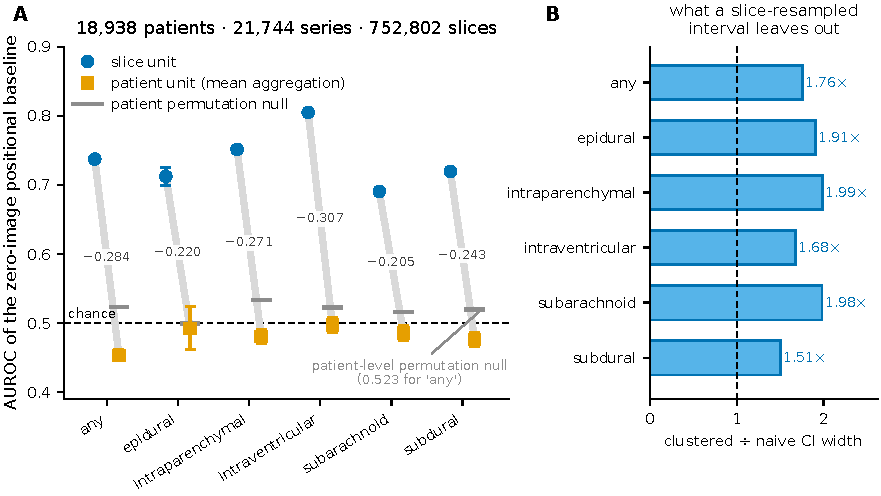
\includegraphics[width=\textwidth]{figures/fig1_collapse.pdf}
\caption{\textbf{One pixel-blind score vector, two units, on RSNA 2019
Intracranial Haemorrhage (\num{752802} slices, \num{18938} patients).}
\textbf{(A)} Slice-level AUROC joined to patient-level AUROC for each of the six
official labels, with 95\% subject-clustered bootstrap intervals and the
within-series permutation null at the patient unit. Nothing changes between the
two readings of a pair except the unit at which the ranking is performed; every
patient-level point estimate lies below chance, and four of the six intervals lie
wholly below it (the epidural and intraventricular intervals cross 0.5).
\textbf{(B)} Width of the correct
subject-clustered interval against the naive slice-resampled interval on the same
six rows: the naive interval is 1.5--2.0 times too narrow.}
\label{fig:collapse}
\end{figure}

\begin{figure}[htbp]
\centering
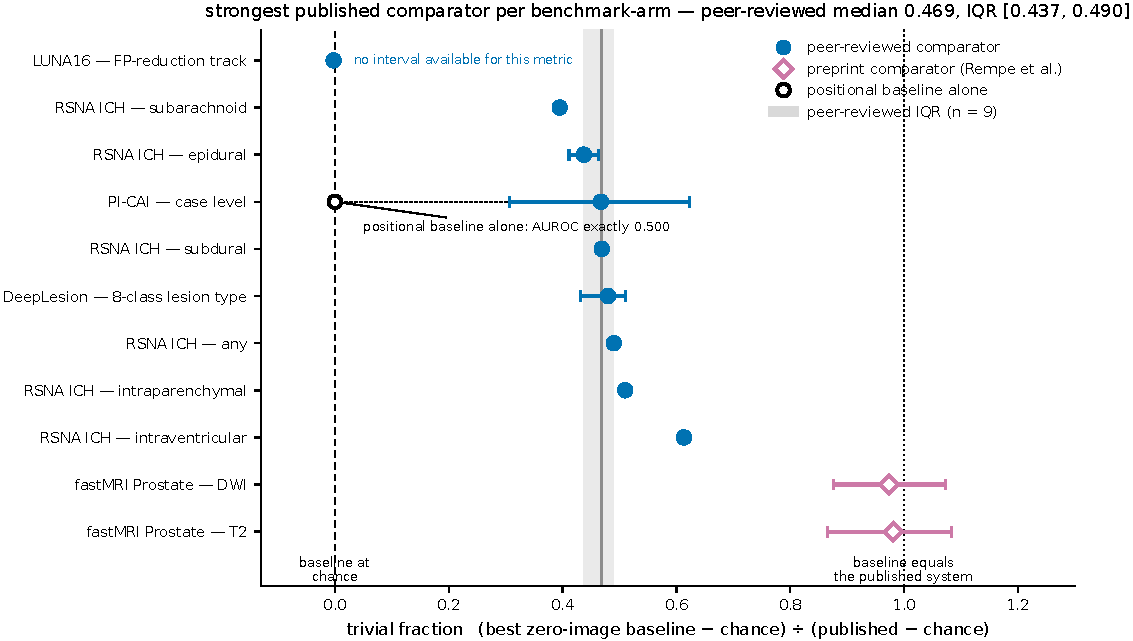
\includegraphics[width=\textwidth]{figures/fig2_trivial_fraction.pdf}
\caption{\textbf{Trivial fraction --- the share of a published margin over chance
reached by a pixel-blind model --- for the strongest published comparator per
benchmark-arm.} Peer-reviewed median 0.469, IQR 0.437--0.490 ($n=9$); the shaded
band is that IQR. Rows whose comparator is an unreviewed preprint are marked as
such and are the only rows reaching 1. The two non-firing benchmark-arms are
plotted at the same prominence as the rest: LUNA16 at $-0.002$ on the challenge's
own competition performance metric, and PI-CAI's positional baseline at exactly
0.500, the correct registration of ``inapplicable''.}
\label{fig:fraction}
\end{figure}

\begin{figure}[htbp]
\centering
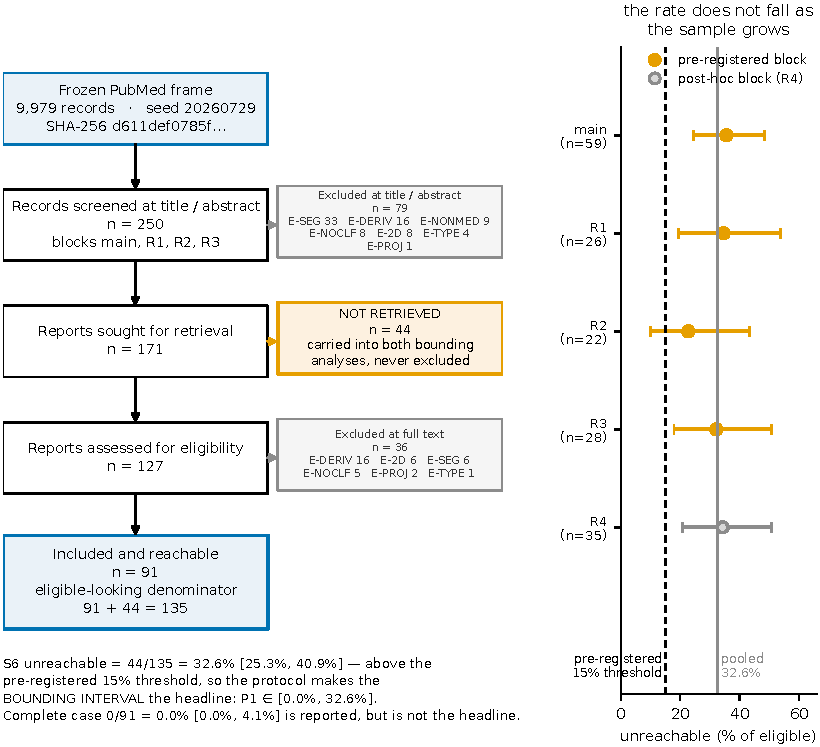
\includegraphics[width=\textwidth]{figures/fig3_prisma_flow.pdf}
\caption{\textbf{Pre-registered prevalence screen: flow and censoring.}
\textbf{(A)} PRISMA 2020 flow adapted for a random-sample meta-research screen:
a frozen \num{9979}-record PubMed frame, 250 records sampled in permutation
order, 79 excluded at title and abstract, 171 reports sought, \textbf{44 not
retrieved and carried into both bounding analyses rather than excluded}, 127
assessed at full text, 36 excluded with reasons, 91 included and reachable. The
eligible-looking denominator is $91+44=135$. \textbf{(B)} Unreachable rate per
screened block against the pre-registered 15\% threshold: the rate does not fall
as the sample grows, which is why the reportable primary result is a bounding
interval rather than a point estimate. The post-hoc fifth block is shown in grey
and is never pooled into the pre-registered denominator.}
\label{fig:prisma}
\end{figure}

\begin{figure}[htbp]
\centering
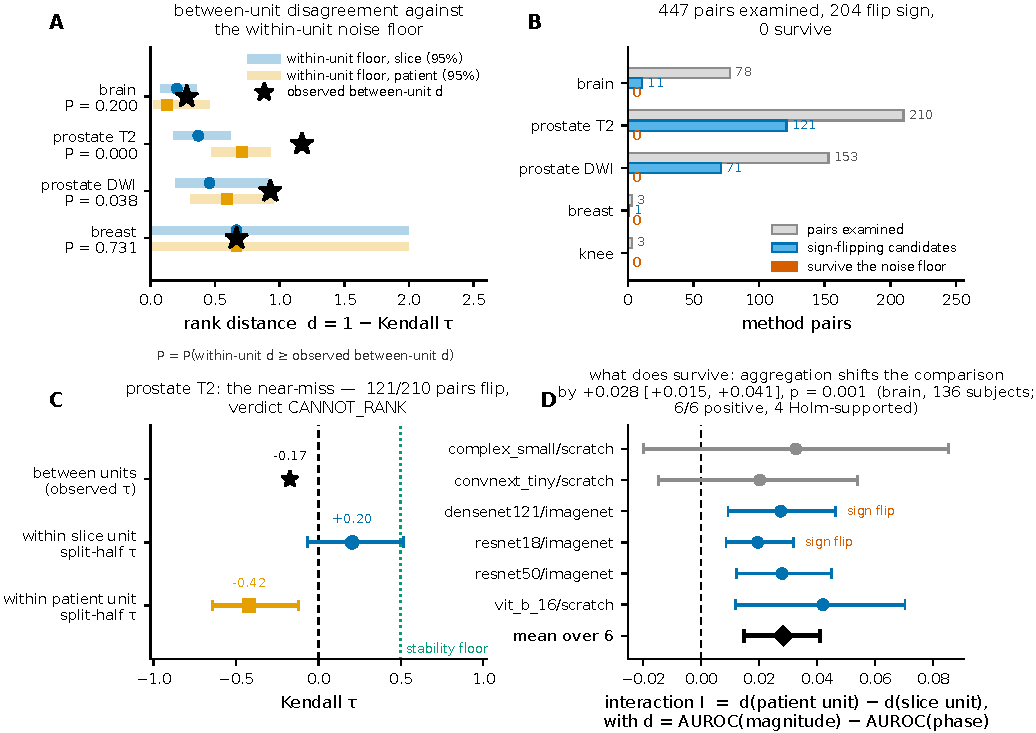
\includegraphics[width=\textwidth]{figures/fig4_rank_inversion.pdf}
\caption{\textbf{Does the evaluation unit change which method wins? A null.}
\textbf{(A)} Observed between-unit rank distance ($D=1-\tau_b$, star) against the
within-unit noise floor produced by resampling subjects with the unit held fixed
(bars, 95\%); $P$ is the fraction of noise-only replicates moving the ranking at
least as far as switching the unit does. \textbf{(B)} Pairs examined,
sign-discordant candidates and survivors after Holm adjustment: 447, 204 and 0.
\textbf{(C)} The near-miss. On prostate T2 the two units share none of their top
three methods and the rank correlation is negative, but two disjoint halves of
the same subjects rank those methods at split-half $\tau=-0.42$ at the patient
unit --- the ranking is not identified, so the disagreement is noise.
\textbf{(D)} What does survive: with architecture held fixed, aggregating from
slice to patient shifts the magnitude-versus-phase comparison by $+0.028$ AUROC
(95\% CI: 0.015, 0.041; $p=0.001$), in the same direction for all six
architectures. The interaction is supported; neither individual ordering is.}
\label{fig:rank}
\end{figure}

\begin{figure}[htbp]
\centering
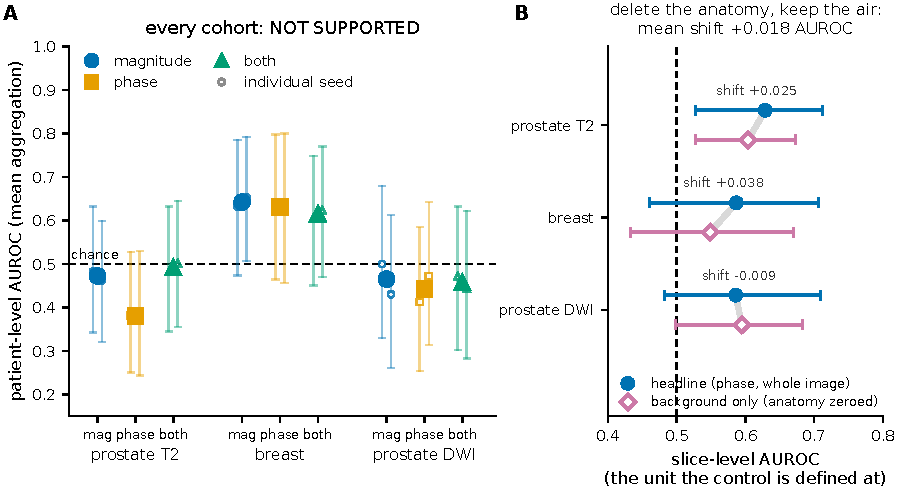
\includegraphics[width=\textwidth]{figures/fig5_case_study.pdf}
\caption{\textbf{The protocol applied to our own study, which it fails.}
\textbf{(A)} Patient-level AUROC with 95\% subject-clustered intervals for
magnitude, phase and both channels on the three clinical cohorts; every cohort is
NOT SUPPORTED against criteria fixed in advance. \textbf{(B)} The background-only
control: deleting the anatomy and training on air alone does not collapse the
slice-level number. A diagnostic signal that survives deleting the patient is not
a diagnostic signal.}
\label{fig:case}
\end{figure}

% =====================================================================
\clearpage
% The .bib file is maintained separately. If it is not yet in the project
% folder this document still compiles, with a placeholder in place of the
% reference list.
\bibliographystyle{unsrtnat}
\bibliography{refs}

\end{document}
